%!TEX TS-program = xelatex

% Шаблон документа LaTeX создан в 2018 году
% Алексеем Подчезерцевым
% В качестве исходных использованы шаблоны
% 	Данилом Фёдоровых (danil@fedorovykh.ru) 
%		https://www.writelatex.com/coursera/latex/5.2.2
%	LaTeX-шаблон для русской кандидатской диссертации и её автореферата.
%		https://github.com/AndreyAkinshin/Russian-Phd-LaTeX-Dissertation-Template

\documentclass[a4paper,14pt]{article}

%%% Работа с русским языком
\usepackage[english,russian]{babel}   %% загружает пакет многоязыковой вёрстки
\usepackage{fontspec}      %% подготавливает загрузку шрифтов Open Type, True Type и др.
\defaultfontfeatures{Ligatures={TeX},Renderer=Basic}  %% свойства шрифтов по умолчанию
\setmainfont[Ligatures={TeX,Historic}]{Times New Roman} %% задаёт основной шрифт документа
\setsansfont{Comic Sans MS}                    %% задаёт шрифт без засечек
\setmonofont{Courier New}
\usepackage{indentfirst}
\frenchspacing

\renewcommand{\epsilon}{\ensuremath{\varepsilon}}
\renewcommand{\phi}{\ensuremath{\varphi}}
\renewcommand{\kappa}{\ensuremath{\varkappa}}
\renewcommand{\le}{\ensuremath{\leqslant}}
\renewcommand{\leq}{\ensuremath{\leqslant}}
\renewcommand{\ge}{\ensuremath{\geqslant}}
\renewcommand{\geq}{\ensuremath{\geqslant}}
\renewcommand{\emptyset}{\varnothing}

%%% Дополнительная работа с математикой
\usepackage{amsmath,amsfonts,amssymb,amsthm,mathtools} % AMS
\usepackage{icomma} % "Умная" запятая: $0,2$ --- число, $0, 2$ --- перечисление

%% Номера формул
%\mathtoolsset{showonlyrefs=true} % Показывать номера только у тех формул, на которые есть \eqref{} в тексте.
%\usepackage{leqno} % Нумерация формул слева	

%% Перенос знаков в формулах (по Львовскому)
\newcommand*{\hm}[1]{#1\nobreak\discretionary{}
{\hbox{$\mathsurround=0pt #1$}}{}}

%%% Работа с картинками
\usepackage{graphicx}  % Для вставки рисунков
\graphicspath{{images/}}  % папки с картинками
\setlength\fboxsep{3pt} % Отступ рамки \fbox{} от рисунка
\setlength\fboxrule{1pt} % Толщина линий рамки \fbox{}
\usepackage{wrapfig} % Обтекание рисунков текстом

%%% Работа с таблицами
\usepackage{array,tabularx,tabulary,booktabs} % Дополнительная работа с таблицами
\usepackage{longtable}  % Длинные таблицы
\usepackage{multirow} % Слияние строк в таблице
\usepackage{float}% http://ctan.org/pkg/float

%%% Программирование
\usepackage{etoolbox} % логические операторы


%%% Страница
\usepackage{extsizes} % Возможность сделать 14-й шрифт
\usepackage{geometry} % Простой способ задавать поля
\geometry{top=20mm}
\geometry{bottom=20mm}
\geometry{left=20mm}
\geometry{right=10mm}
%
%\usepackage{fancyhdr} % Колонтитулы
% 	\pagestyle{fancy}
%\renewcommand{\headrulewidth}{0pt}  % Толщина линейки, отчеркивающей верхний колонтитул
% 	\lfoot{Нижний левый}
% 	\rfoot{Нижний правый}
% 	\rhead{Верхний правый}
% 	\chead{Верхний в центре}
% 	\lhead{Верхний левый}
%	\cfoot{Нижний в центре} % По умолчанию здесь номер страницы

\usepackage{setspace} % Интерлиньяж
\onehalfspacing % Интерлиньяж 1.5
%\doublespacing % Интерлиньяж 2
%\singlespacing % Интерлиньяж 1

\usepackage{lastpage} % Узнать, сколько всего страниц в документе.

\usepackage{soul} % Модификаторы начертания

\usepackage{hyperref}
\usepackage[usenames,dvipsnames,svgnames,table,rgb]{xcolor}
\hypersetup{                % Гиперссылки
unicode=true,           % русские буквы в раздела PDF
pdftitle={Заголовок},   % Заголовок
pdfauthor={Автор},      % Автор
pdfsubject={Тема},      % Тема
pdfcreator={Создатель}, % Создатель
pdfproducer={Производитель}, % Производитель
pdfkeywords={keyword1}, % Ключевые слова
colorlinks=true,        % false: ссылки в рамках; true: цветные ссылки
linkcolor=black,          % внутренние ссылки
citecolor=black,        % на библиографию
filecolor=magenta,      % на файлы
urlcolor=blue           % на URL
}
\makeatletter
\def\@biblabel#1{#1. }
\makeatother
\usepackage{cite} % Работа с библиографией
%\usepackage[superscript]{cite} % Ссылки в верхних индексах
%\usepackage[nocompress]{cite} % 
\usepackage{csquotes} % Еще инструменты для ссылок

\usepackage{multicol} % Несколько колонок

\usepackage{tikz} % Работа с графикой
\usepackage{pgfplots}
\usepackage{pgfplotstable}

% ГОСТ заголовки
\usepackage[font=small]{caption}
%\captionsetup[table]{justification=centering, labelsep = newline} % Таблицы по правобу краю
%\captionsetup[figure]{justification=centering} % Картинки по центру


\newcommand{\tablecaption}[1]{\addtocounter{table}{1}\small \begin{flushright}
                                                                \tablename \ \thetable
\end{flushright}%
\begin{center}
    #1
\end{center}}

\newcommand{\imref}[1]{рис.~\ref{#1}}

\usepackage{multirow}
\usepackage{spreadtab}
\newcolumntype{K}[1]{@{}>{\centering\arraybackslash}p{#1cm}@{}}


\usepackage{xparse}
\usepackage{fancyvrb}

\RecustomVerbatimCommand{\VerbatimInput}{VerbatimInput}
{
fontsize=\footnotesize
}

\usepackage{tocloft}
\renewcommand{\cftsecleader}{\cftdotfill{\cftdotsep}}
\begin{document} % конец преамбулы, начало документа
    \begin{titlepage}
    \begin{center}
        ФЕДЕРАЛЬНОЕ ГОСУДАРСТВЕННОЕ АВТОНОМНОЕ \\
        ОБРАЗОВАТЕЛЬНОЕ УЧРЕЖДЕНИЕ ВЫСШЕГО ОБРАЗОВАНИЯ\\
        «НАЦИОНАЛЬНЫЙ ИССЛЕДОВАТЕЛЬСКИЙ УНИВЕРСИТЕТ\\
        «ВЫСШАЯ ШКОЛА ЭКОНОМИКИ»
    \end{center}

    \begin{center}
        \textbf{Московский институт электроники и математики}

        \textbf{им. А.Н.Тихонова НИУ ВШЭ}

        \vspace{2ex}

        \textbf{Департамент компьютерной инженерии}
    \end{center}
    \vspace{1ex}

    \begin{center}
        Курс «Высокоуровневое и имитационное моделирование цифровых систем»
    \end{center}


    \begin{center}
        \textbf{ОТЧЕТ\\
        ПО ЛАБОРАТОРНОЙ РАБОТЕ №3
        }
    \end{center}

    \begin{center}
        Тема работы: «Реализация нейронной сети MobileNet на ПЛИС»
    \end{center}

    \vspace{2ex}

    \begin{flushright}
        \textbf{Выполнили:}

        \vspace{2ex}

        Студенты группы БИВ174

        Бригада №5

        \vspace{2ex}

        Подчезерцев Алексей Евгеньевич

        Солодянкин Андрей Александрович
        \vspace{2ex}

        \textbf{Принял:}

        асс. МИЭМ НИУ ВШЭ

        Американов А.А.

    \end{flushright}

    \vfill
    \begin{center}
        Москва \the\year \, г.
    \end{center}

\end{titlepage}
\addtocounter{page}{1}
    \tableofcontents
    \pagebreak


    \section{Задание}

    Бригада №5.

    MAX 10 NEEK

    \begin{enumerate}
        \item Ознакомиться с примерами использования DPI и PLI/VPI;
        \item Создать дешифратор 17 разрядный с использованием DPI;
        \item Создать функцию, изменяющую четные числа в массиве на 1.
    \end{enumerate}


    \section{Выполнение работы}

    \subsection{Задание №5}

    Была выполнена программа examples/tutorials/systemverilog/dpi\_basic/.
    Результат представлен на рис.~\ref{fig:05_wave}.
    Сначала включается цвет по умолчанию -- красный, затем включается зеленый, после управление передается в С код.
    В C коде печатается сообщение, включается желтый свет, вызывается функция $sv\_WaitForRed$, которая ожидает 10нс,
    после включается красный свет, управление возвращается в SystemVerilog.
    Через 10нс снова включается зеленый.

    Фрагмент SystemVerilog теста.
    {\small \VerbatimInput{code/05_test.sv}}

    Фрагмент C кода.
    {\small \VerbatimInput{code/05_foreign.c}}

    \begin{figure}[H]
        \centering
        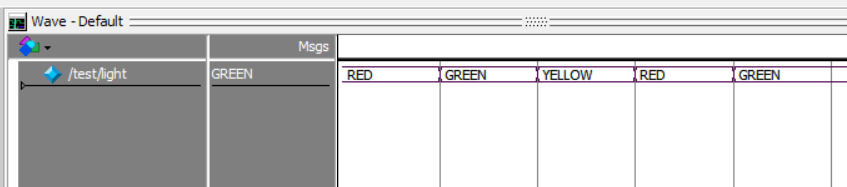
\includegraphics[width=\linewidth]{images/05_wave}
        \caption{Вейвформа для dpi\_basic}
        \label{fig:05_wave}
    \end{figure}

    \subsection{Задание №6}

    Был изучен пример examples/systemverilog/dpi/dpivpipert.
    В данном примере сравниваются подходы PLI/VPI и DPI.

    Первый подход требует большое число кода для генерации и регистрации функций, объявлении стандартных полей.
    DPI же лаконичен и довольно прост, не требует большого числа кода
    DPI является развитием PLI/VPI, логичнее использовать его.

    \subsection{Задание №7}

    Был изучен пример examples/systemverilog/dpi/simple\_calls.

    В данном примере показываются способы вызова C методов из SystemVerilog и наоборот.

    Исходный код С:
    {\small \VerbatimInput{code/07_cimports.c}}

    Исходный код SystemVerilog:
    {\small \VerbatimInput{code/07_simple_calls.sv}}

    Результат выполнения:
    {\small \VerbatimInput{code/07_results.txt}}

    \subsection{Задание №8}

    Был изучен пример examples/systemverilog/dpi/openarray.

    В данном примере демонстрируются различные способы обработки массивов различной размерности.
    Данный подход был использован в работе.

    Результат выполнения:
    {\small \VerbatimInput{code/08_logs.txt}}

    \subsection{Задание №9}

    Был изучен пример examples/systemverilog/dpi/packed\_types.

    Результат выполнения:
    {\small \VerbatimInput{code/09_packed_logs.txt}}

    Был изучен пример examples/systemverilog/dpi/unpacked\_types.

    Результат выполнения:
    {\small \VerbatimInput{code/09_unpacked_logs.txt}}

    При передаче неупакованных данных требуется дополнительно совершать операции упаковки и распаковки.

    \subsection{Задание №10}

    Был изучен пример examples/systemverilog/dpi/checkpoint.

    Данная технология может применяться для выполнения теста с некоторого ненулевого этапа,
    например -- для пропуска длительных этапов.

    \subsection{Задание №11}

    Был изучен пример examples/systemverilog/dpi/cpackages.

    В данном примере изучаются различные способы выполнения команд и проверки их статуса.

    \subsection{Задание №12}

    Был изучен пример examples/systemverilog/dpi/create\_sv\_dynarray.

    Данная технология может применяться для работы с массивами неизвестной начальной длины.


    \section{Самостоятельная работа}

    \subsection{Мультиплексор}

    Была выполнена программа examples/systemverilog/dpi/mux81.
    Корректный результат работы представлен на рис.~\ref{fig:02_mux_ok}.

    \begin{figure}[H]
        \centering
        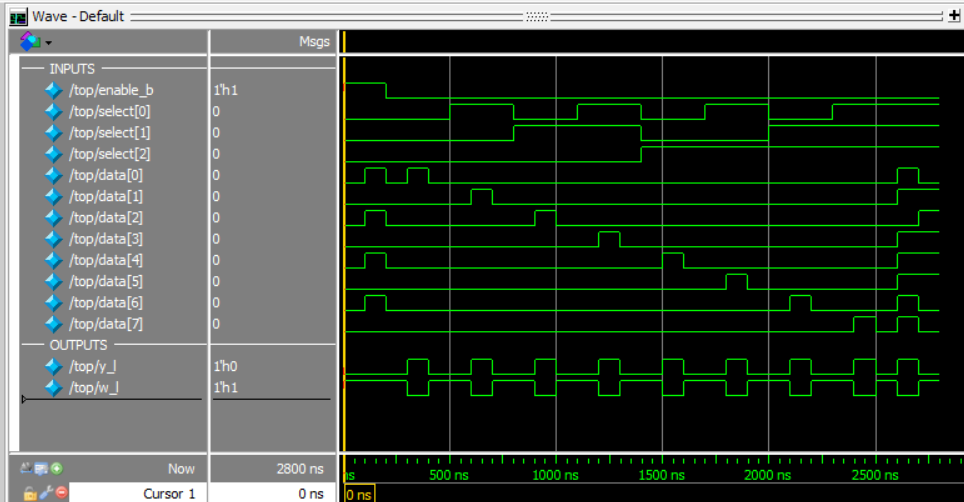
\includegraphics[width=\linewidth]{images/02_mux_ok}
        \caption{Корректная работа мультиплексора}
        \label{fig:02_mux_ok}
    \end{figure}

    Далее были поданы некоторые сигналы равные b или z.
    Результат работы представлен на рис.~\ref{fig:02_mux_bz}.
    Вывод программы:
    {\small \VerbatimInput{code/02_mux_bz.txt}}

    \begin{figure}[H]
        \centering
        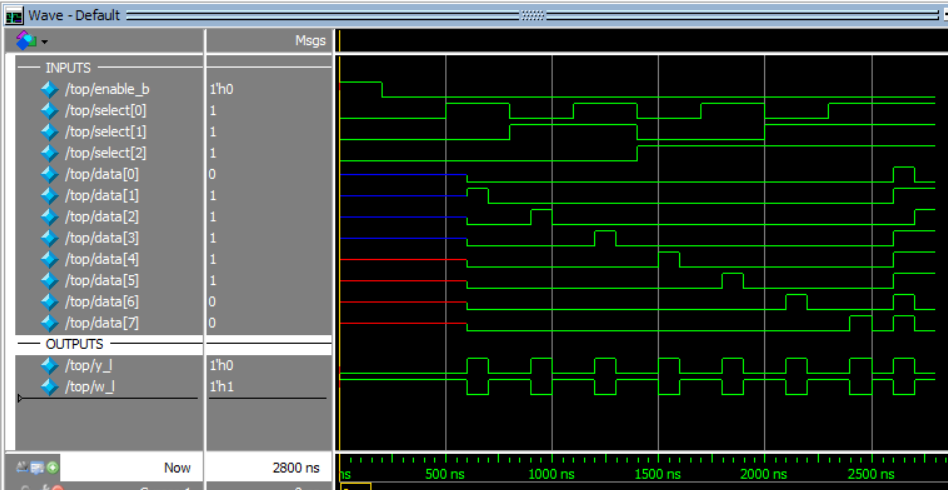
\includegraphics[width=\linewidth]{images/02_mux_bz}
        \caption{Подача b и z на мультиплексор}
        \label{fig:02_mux_bz}
    \end{figure}

    После была внесена ошибка в обработку сигналов мультиплексора.
    Результат работы представлен на рис.~\ref{fig:02_mux_error}.
    Вывод программы:
    {\small \VerbatimInput{code/02_mux_error.txt}}

    \begin{figure}[H]
        \centering
        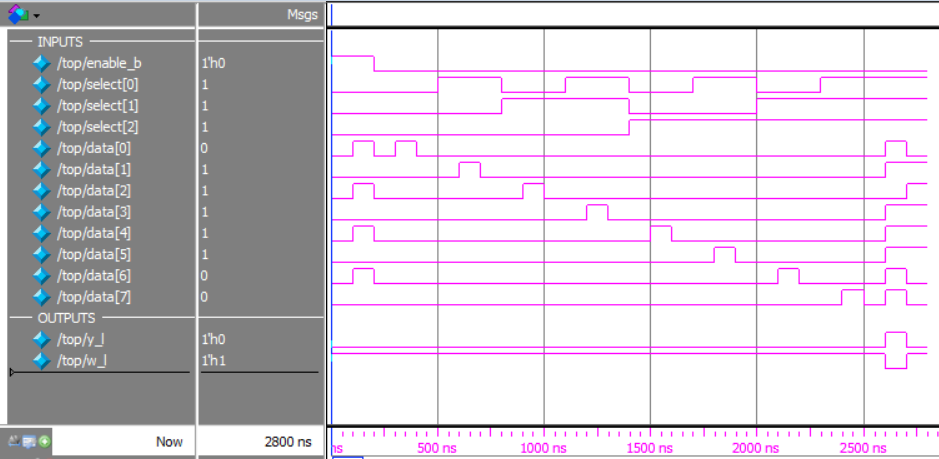
\includegraphics[width=\linewidth]{images/02_mux_error}
        \caption{Ошибка мультиплексора}
        \label{fig:02_mux_error}
    \end{figure}

    \subsection{Дешифратор}

    В соответствии с заданием был разработан дешифратор 17 разрядный.
    Вейвформа представлена на рис.~\ref{fig:02_decoder}.

    Исходный код C:
    {\small \VerbatimInput{../decoder/decoder.c}}

    Исходный код Verilog модуля:
    {\small \VerbatimInput{../decoder/decoder17.v}}

    Исходный код тестирования Verilog модуля:
    {\small \VerbatimInput{../decoder/decoder17_test.v}}

    \begin{figure}[H]
        \centering
        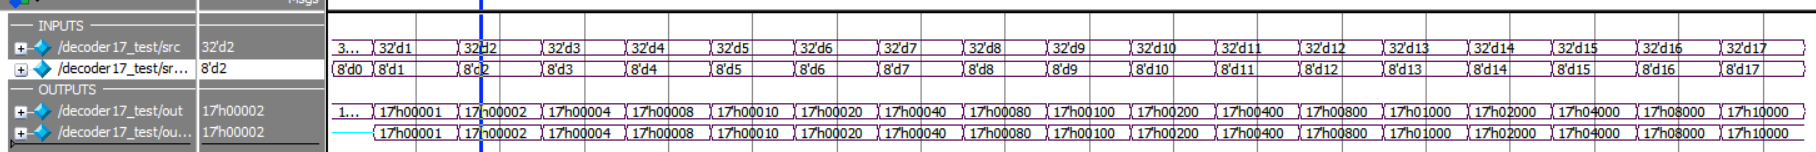
\includegraphics[width=\linewidth]{images/02_decoder}
        \caption{Результат работы декодера}
        \label{fig:02_decoder}
    \end{figure}

    Результат работы программы:
    {\small \VerbatimInput{code/02_decoder_ok.txt}}

    В исходный код была внесена ошибка, появились отличия в работе программы.
    {\small \VerbatimInput{code/02_decoder_error.txt}}

    \subsection{Последовательность Фибоначчи}

    Была выполнена программа examples/systemverilog/dpi/fibonacci.
    Корректный результат работы представлен на рис.~\ref{fig:03_fib}.

    \begin{figure}[H]
        \centering
        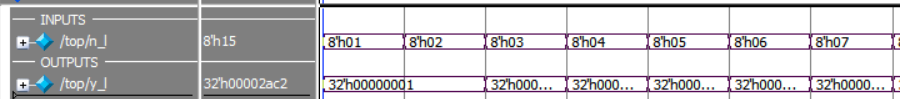
\includegraphics[width=\linewidth]{images/03_fib}
        \caption{Корректная работа последовательности Фибоначчи}
        \label{fig:03_fib}
    \end{figure}

    В программу была внесена ошибка, после чего появились множественные ошибки:
    {\small \VerbatimInput{code/03_fib_error.txt}}

    Далее функция была переписана в рекурсивном варианте:
    {\small \VerbatimInput{../fibonacci/fibonacci.c}}

    Полученный вариант прошел тесты.

    \subsection{Работа с массивами}

    Необходимо изменить исходный массив таким образом, что все четные элементы заменяются 1.
    Вейвформа представлена на рис.~\ref{fig:04_extra}.
    Можно заметить баг вейвформы -- в консоли результат отображается корректно.

    Исходный код C:
    {\small \VerbatimInput{../extra/extra.c}}

    Исходный код тестирования модуля:
    {\small \VerbatimInput{../extra/extra_test.v}}

    \begin{figure}[H]
        \centering
        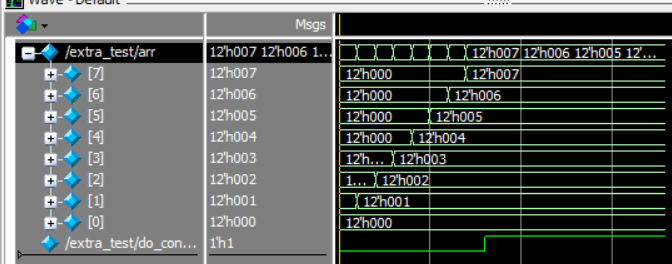
\includegraphics[width=\linewidth]{images/04_extra}
        \caption{Результат работы программы}
        \label{fig:04_extra}
    \end{figure}

    Результат работы программы:
    {\small \VerbatimInput{code/04_extra.txt}}


    \section{Исходные коды}

    Исходные коды доступны на \href{https://github.com/AsciiShell/hse_hlimds_labs}
    {https://github.com/AsciiShell/hse\_hlimds\_labs}.

    Pull request работы \href{https://github.com/AsciiShell/hse_hlimds_labs/pull/4}
    {https://github.com/AsciiShell/hse\_hlimds\_labs/pull/4}.


    \section{Выводы по работе}

    В ходе работы был изучены технологии DPI и PLI/VPI, их отличия.
    Был получен опыт написания C методов, передачи данных и вызовов C кода из SystemVerilog и наоборот.
    Были написаны самостоятельно модули для верификации работы некоторых устройств и проверки их работы на наличие ошибок.

\end{document} % конец документа
